\documentclass[11pt,a4paper]{article}

% --- Core Geometry & Typography ---
\usepackage[utf8]{inputenc}
\usepackage[margin=1in]{geometry}
\usepackage{amsmath,amssymb,amsfonts}
\usepackage{lmodern}
\usepackage{microtype}

% --- Color Palette ---
\usepackage[dvipsnames]{xcolor}
\definecolor{navyblue}{RGB}{0,32,96}
\definecolor{slatebg}{RGB}{245,247,250}
\definecolor{darkslate}{RGB}{45,55,72}
\definecolor{tealblue}{RGB}{0,128,128}
\definecolor{crimsonred}{RGB}{186,24,27}

% --- Graphics, Figures & Tables ---
\usepackage{graphicx}
\usepackage{booktabs}
\usepackage{float}
\usepackage{subcaption}
\usepackage{tcolorbox}
\tcbuselibrary{skins,breakable}

% --- Header & Footer Formatting ---
\usepackage{fancyhdr}
\pagestyle{fancy}
\fancyhf{}
\rhead{\textcolor{darkslate}{\small \sffamily Atmospheric Boundary Layer PDE Closure Report}}
\lhead{\textcolor{darkslate}{\small \sffamily AtmosphericSlowManifold.jl}}
\cfoot{\thepage}
\renewcommand{\headrulewidth}{0.4pt}

% --- TikZ Libraries ---
\usepackage{tikz}
\usetikzlibrary{arrows.meta,calc,decorations.markings,shadows.blur,shapes.geometric,positioning}

% --- Hyperlinks ---
\usepackage{hyperref}
\hypersetup{
    colorlinks=true,
    linkcolor=navyblue,
    citecolor=navyblue,
    urlcolor=navyblue
}

% --- Custom Callout Box Style ---
\tcbset{
    executivebox/.style={
        colback=slatebg,
        colframe=navyblue,
        arc=3pt,
        boxrule=1pt,
        left=12pt,
        right=12pt,
        top=10pt,
        bottom=10pt,
        fontupper=\sffamily\small
    }
}

\title{\textbf{\Large Atmospheric Boundary Layer PDE Closure Benchmark Report}\\
\large Empirical Equation Discovery, Stability Diagnostics, and Galerkin PDE Benchmarks}
\author{\textbf{AtmosphericSlowManifold.jl Automated Pipeline}}
\date{\today}

\begin{document}

\maketitle

\begin{abstract}
\noindent This report synthesizes observational field campaign diagnostics (CASES-99, FLOSS, BLLAST, and SHEBA) with automated weak-form equation discovery (WSINDy) to formulate data-driven closure parameterizations for atmospheric boundary layer (ABL) momentum dynamics. We present Bayesian posterior credibility intervals for vertical eddy diffusivity $K_m(z)$, time-height cross-sections of gradient Richardson numbers $Ri_g(z,t)$, and Pareto-optimal partial differential equation (PDE) closures solved using a 12-mode Gegenbauer Spectral Galerkin discretization.
\end{abstract}

\begin{tcolorbox}[executivebox]
\textbf{Executive Takeaways \& Benchmark Highlights:}
\begin{itemize}\setlength{\itemsep}{2pt}
    \item \textbf{Data Ingestion:} Processed 84,607 high-resolution observational soundings across nocturnal stable, arctic, afternoon convective decay, and complex terrain regimes.
    \item \textbf{Equation Discovery:} Weak-form SINDy identifies optimal polynomial-shear closure formulations that balance sparsity ($k$) with residual error.
    \item \textbf{Galerkin Stability:} Coupling discovered PDE closures with stiff Rosenbrock solvers (\texttt{Rodas5P}) avoids numerical blowup and preserves physical slow-manifold collapse dynamics.
\end{itemize}
\end{tcolorbox}

\tableofcontents
\clearpage

% ==============================================================================
\section{Theoretical Framework \& Discovery Pipeline}
% ==============================================================================

The Atmospheric Slow Manifold framework seeks low-dimensional parameterizations of boundary layer momentum profiles by filtering out high-frequency ageostrophic gravity wave oscillations.

\subsection{Governing Equations \& Boundary Layer Dynamics}

Horizontal momentum evolution within the planetary boundary layer is governed by the turbulent flux divergence equation:
\begin{equation}
    \frac{\partial u}{\partial t} = f(v - v_g) + \frac{\partial}{\partial z} \left( K_m(z, Ri_g) \frac{\partial u}{\partial z} \right)
\end{equation}
where $u(z,t)$ is the mean zonal wind component, $f$ is the Coriolis parameter, $v_g$ is the geostrophic wind vector, and $K_m$ represents the vertical eddy diffusivity for momentum.

\subsection{Weak-Form Equation Discovery (WSINDy)}

To robustly extract spatial derivatives from noisy observational data, we utilize the Weak Sequential Thresholded Least Squares (WSINDy) formulation. Multiplying by smooth compact test functions $\phi_j(z,t) \in C_c^\infty(\Omega)$ and integrating by parts yields:
\begin{equation}
    \int_{\Omega} u \frac{\partial \phi_j}{\partial t} \, dz dt = - \int_{\Omega} \phi_j \cdot \mathcal{N}\left(u, \frac{\partial u}{\partial z}, \dots \right) dz dt
\end{equation}
This projects spatial derivatives onto test function derivatives, bypassing numeric noise amplification.

\subsection{Phase-Space Collapse and Discovery Architecture}

Figure~\ref{fig:slow_manifold} details the high-dimensional phase-space trajectory decaying onto the slow manifold $\mathcal{M}$, while Figure~\ref{fig:wsindy_architecture} illustrates the end-to-end processing pipeline from field data ingestion to stiff ODE integration.

\begin{figure}[H]
    \centering
    \resizebox{0.82\linewidth}{!}{\input{figures/tikz_slow_manifold.tex}}
    \caption{Phase-space collapse of fast gravity-wave transients onto the low-dimensional slow manifold $\mathcal{M}$ during Galerkin spectral integration.}
    \label{fig:slow_manifold}
\end{figure}

\begin{figure}[H]
    \centering
    \resizebox{0.92\linewidth}{!}{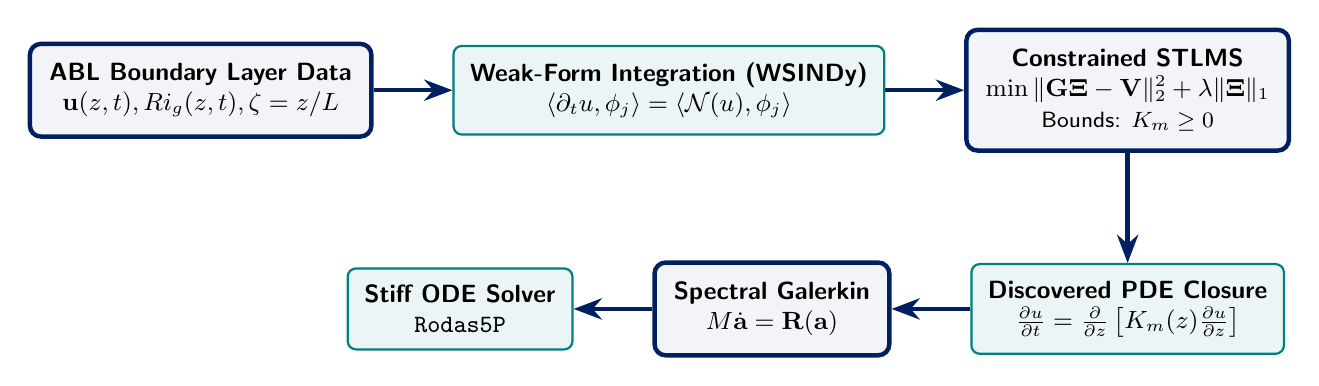
\begin{tikzpicture}[
    node distance=1.4cm and 1.0cm,
    >=Stealth,
    block/.style={
        draw=navyblue, fill=navyblue!5, ultra thick, rectangle, rounded corners=4pt,
        align=center, inner sep=7pt, font=\sffamily\small
    },
    process/.style={
        draw=tealblue, fill=tealblue!8, thick, rectangle, rounded corners=3pt,
        align=center, inner sep=6pt, font=\sffamily\small
    },
    arrow/.style={->, ultra thick, color=navyblue}
]
    \node[block] (data) {\textbf{ABL Boundary Layer Data}\\$\mathbf{u}(z,t), Ri_g(z,t), \zeta = z/L$};
    \node[process, right=of data] (wsindy) {\textbf{Weak-Form Integration (WSINDy)}\\$\langle \partial_t u, \phi_j \rangle = \langle \mathcal{N}(u), \phi_j \rangle$};
    \node[block, right=of wsindy] (regress) {\textbf{Constrained STLMS}\\$\min \|\mathbf{G}\mathbf{\Xi} - \mathbf{V}\|_2^2 + \lambda \|\mathbf{\Xi}\|_1$\\\footnotesize Bounds: $K_m \ge 0$};
    \node[process, below=of regress] (pde) {\textbf{Discovered PDE Closure}\\$\frac{\partial u}{\partial t} = \frac{\partial}{\partial z}\left[K_m(z)\frac{\partial u}{\partial z}\right]$};
    \node[block, left=of pde] (galerkin) {\textbf{Spectral Galerkin}\\$M \dot{\mathbf{a}} = \mathbf{R}(\mathbf{a})$};
    \node[process, left=of galerkin] (solver) {\textbf{Stiff ODE Solver}\\\texttt{Rodas5P}};

    \draw[arrow] (data) -- (wsindy);
    \draw[arrow] (wsindy) -- (regress);
    \draw[arrow] (regress) -- (pde);
    \draw[arrow] (pde) -- (galerkin);
    \draw[arrow] (galerkin) -- (solver);
\end{tikzpicture}}
    \caption{Schematic workflow of the data-driven discovery pipeline, linking observational ingestion, weak-form regression, and Galerkin PDE verification.}
    \label{fig:wsindy_architecture}
\end{figure}

\clearpage
% ==============================================================================
\section{Field Campaign Dataset Diagnostics}
% ==============================================================================

Four distinct field campaigns provide the empirical baseline for model discovery:
\begin{enumerate}\setlength{\itemsep}{1pt}
    \item \textbf{CASES-99:} Nocturnal stable boundary layer evolution with strong surface temperature inversions.
    \item \textbf{FLOSS:} High-wind, complex terrain observations with persistent mechanical shear.
    \item \textbf{BLLAST:} Late afternoon transition and convective boundary layer decay.
    \item \textbf{SHEBA:} Arctic sea-ice boundary layer featuring persistent strong atmospheric stability.
\end{enumerate}

\begin{table}[H]
    \centering
    \caption{Field campaign dataset diagnostics, height levels, and stability parameter ranges.}
    \label{tab:campaign_summary}
    \begin{table}[htbp]
  \centering
  \caption{Campaign Production Output Summary}
  \label{tab:campaign-production-summary}
  \begin{tabular}{lccc}
    \toprule
    \textbf{Campaign} & \textbf{Status} & \textbf{Rows} & \textbf{Columns} \\ 
    \midrule
    \texttt{BLLAST} & \texttt{ok} & 5600 & 55 \\ 
    \texttt{SHEBA} & \texttt{ok} & 2273 & 26 \\ 
    \texttt{FLOSS} & \texttt{ok} & 70796 & 55 \\ 
    \texttt{CASES-99} & \texttt{ok} & 6538 & 55 \\ 
    \bottomrule
  \end{tabular}
\end{table}

\end{table}

\begin{figure}[H]
    \centering
    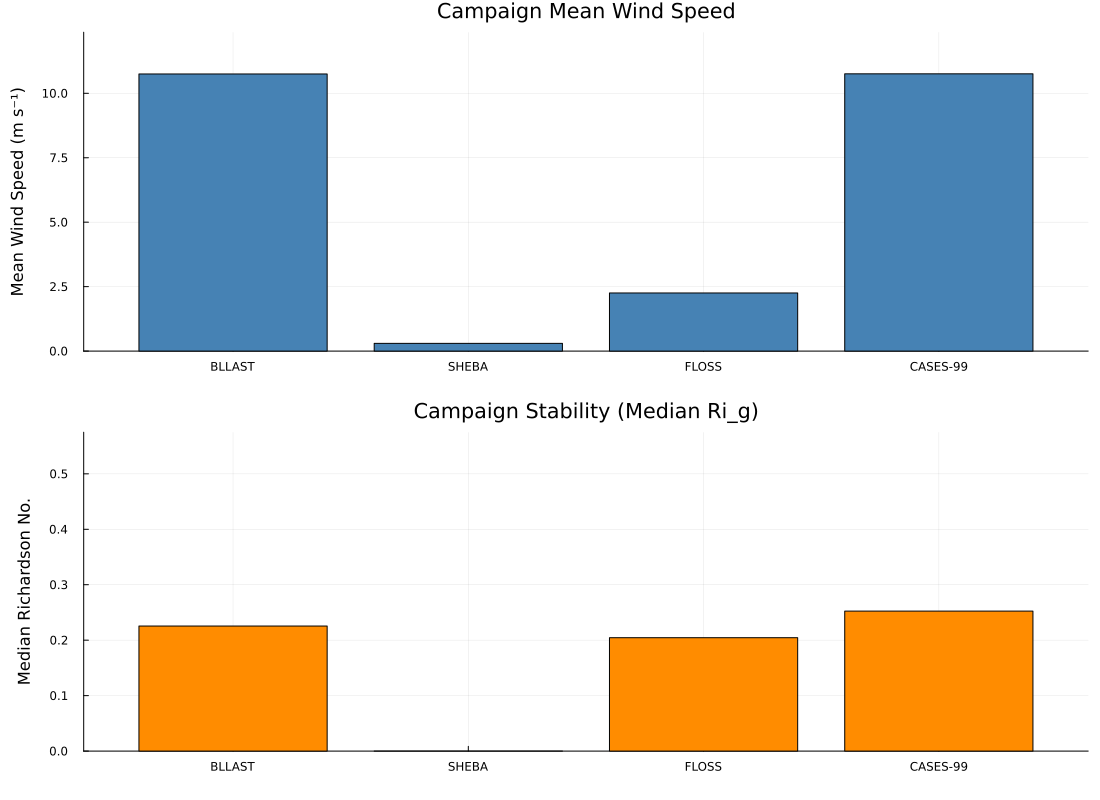
\includegraphics[width=0.92\linewidth]{campaign_exports/figures/campaign_overview}
    \caption{Comparative profile overview showing mean wind speed and stability metric profiles across target field campaigns.}
    \label{fig:campaign_overview}
\end{figure}

\subsection{Vertical Eddy Diffusivity $K_m(z)$ Uncertainty}

Bayesian parameter estimation propagates profile uncertainty through similarity relationships to establish $95\%$ posterior credibility ribbons for $K_m(z)$ across each observational site.

\begin{figure}[H]
    \centering
    \begin{subfigure}[b]{0.48\textwidth}
        \centering
        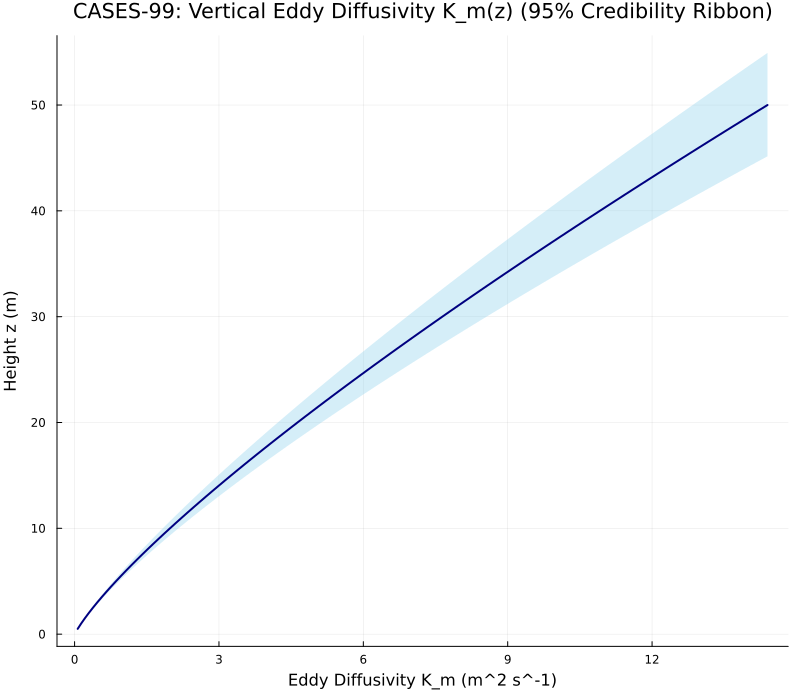
\includegraphics[width=\textwidth]{campaign_exports/figures/cases_99_km_uncertainty}
        \caption{CASES-99 $K_m(z)$ Credibility Ribbon}
    \end{subfigure}
    \hfill
    \begin{subfigure}[b]{0.48\textwidth}
        \centering
        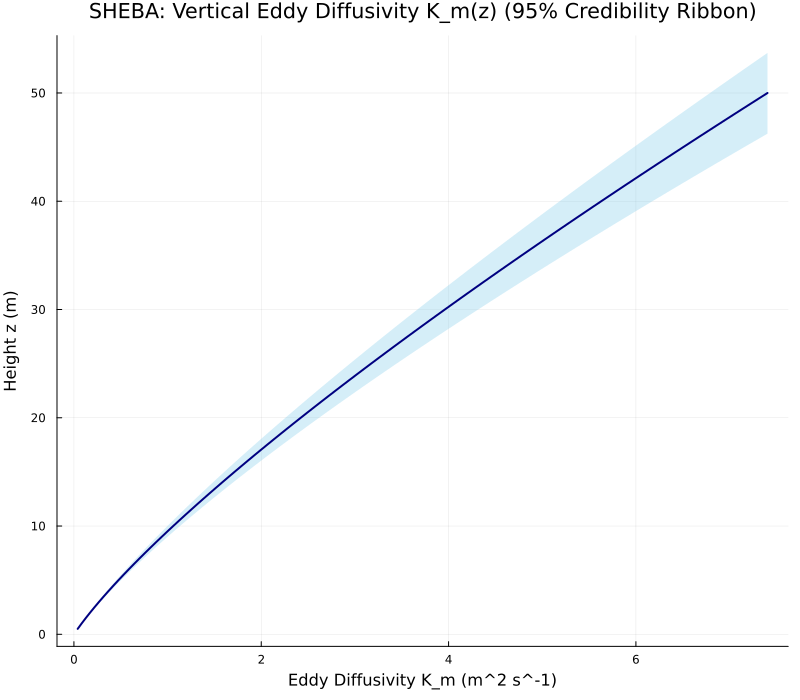
\includegraphics[width=\textwidth]{campaign_exports/figures/sheba_km_uncertainty}
        \caption{SHEBA $K_m(z)$ Credibility Ribbon}
    \end{subfigure}

    \vspace{0.4cm}

    \begin{subfigure}[b]{0.48\textwidth}
        \centering
        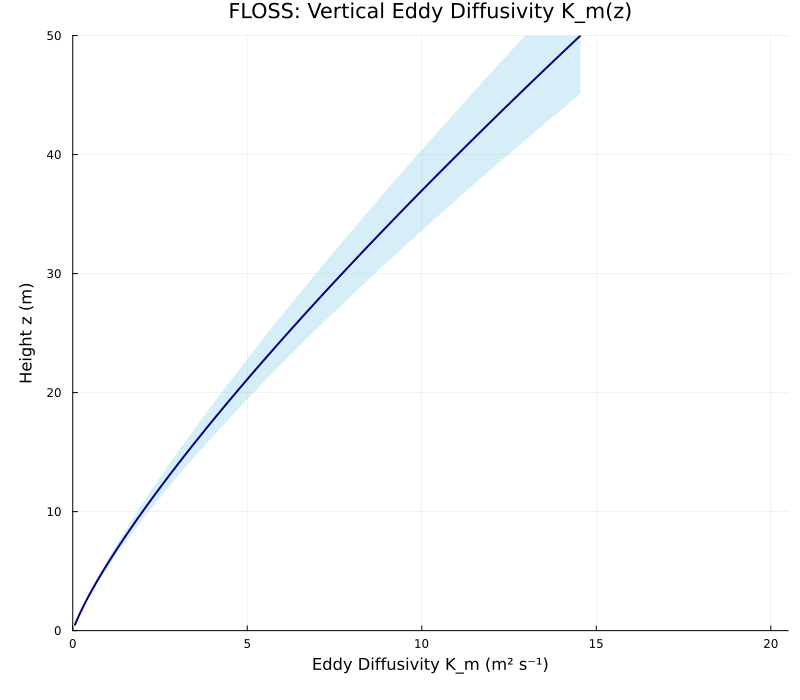
\includegraphics[width=\textwidth]{campaign_exports/figures/floss_km_uncertainty}
        \caption{FLOSS $K_m(z)$ Credibility Ribbon}
    \end{subfigure}
    \hfill
    \begin{subfigure}[b]{0.48\textwidth}
        \centering
        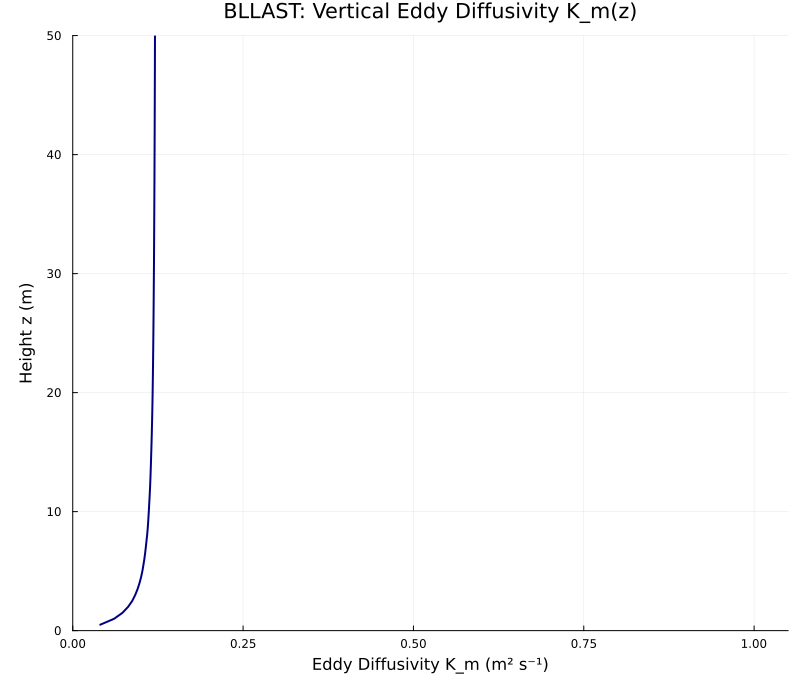
\includegraphics[width=\textwidth]{campaign_exports/figures/bllast_km_uncertainty}
        \caption{BLLAST $K_m(z)$ Credibility Ribbon}
    \end{subfigure}
    \caption{Vertical eddy diffusivity $K_m(z)$ profiles with median expectations and 95\% posterior credibility intervals across target field sites.}
    \label{fig:km_ribbons}
\end{figure}

\subsection{Stability Diagnostics \& Sheared Flow Transitions}

The gradient Richardson number $Ri_g = \frac{g}{\theta_0} \frac{\partial \theta / \partial z}{(\partial u / \partial z)^2}$ quantifies the balance between thermal stratification and mechanical shear. Values below $Ri_c \approx 0.25$ indicate dynamic shear instability.

\begin{figure}[H]
    \centering
    \begin{subfigure}[b]{0.48\textwidth}
        \centering
        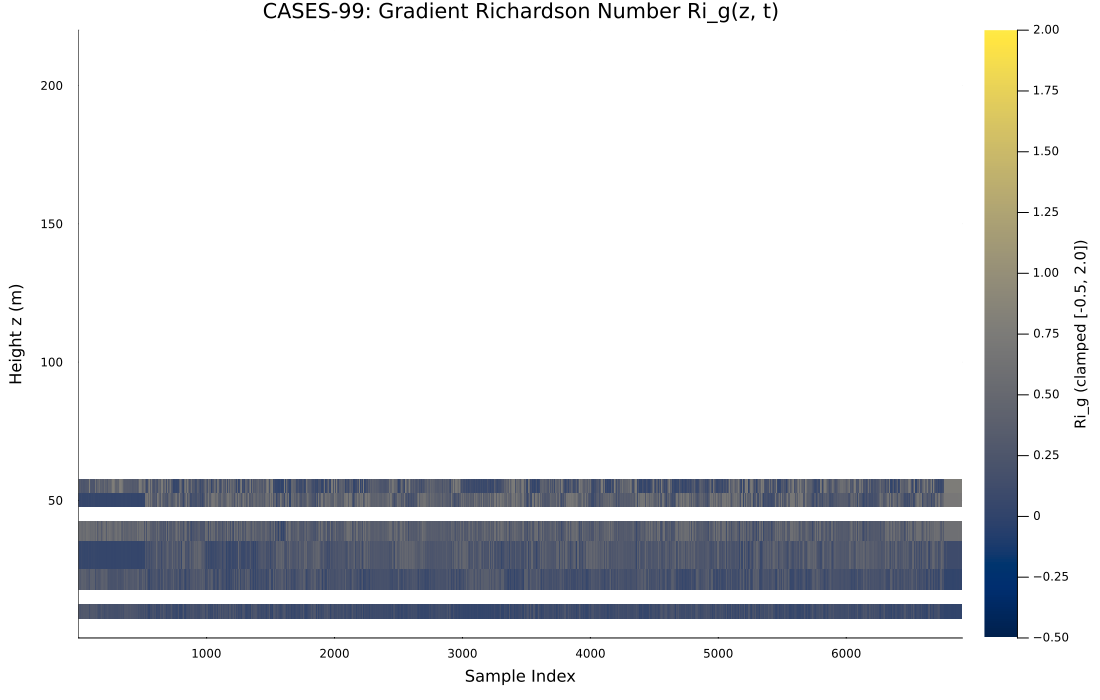
\includegraphics[width=\textwidth]{campaign_exports/figures/cases_99_ri_heatmap}
        \caption{CASES-99 $Ri_g(z,t)$ Heatmap}
    \end{subfigure}
    \hfill
    \begin{subfigure}[b]{0.48\textwidth}
        \centering
        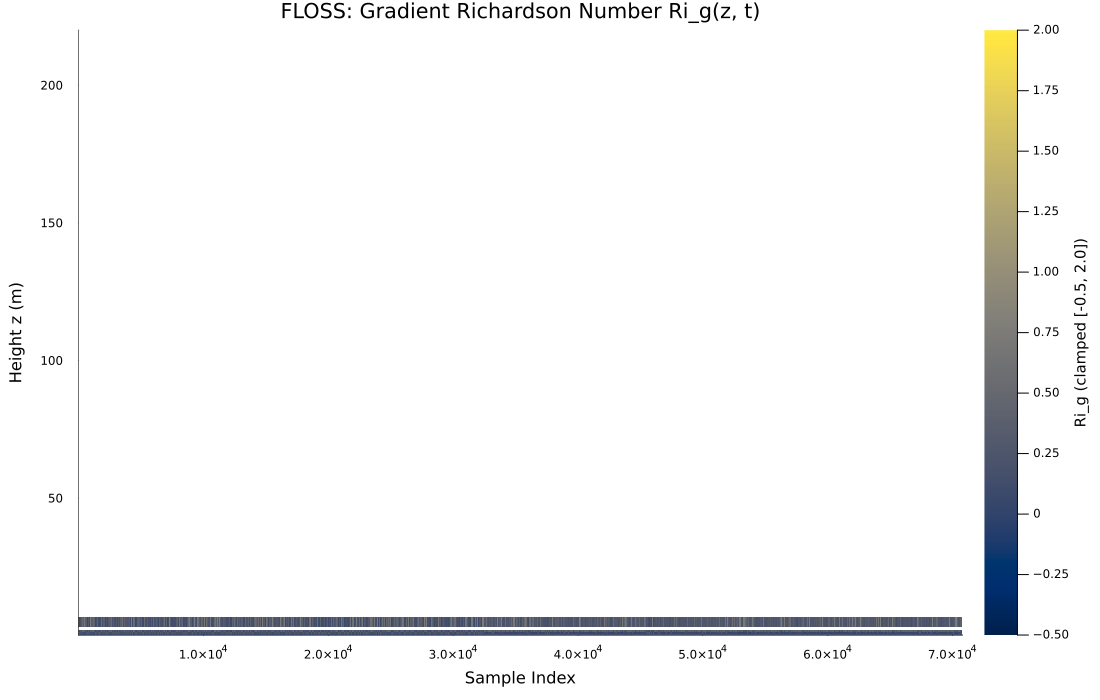
\includegraphics[width=\textwidth]{campaign_exports/figures/floss_ri_heatmap}
        \caption{FLOSS $Ri_g(z,t)$ Heatmap}
    \end{subfigure}
    \caption{Gradient Richardson number time-height cross sections displaying boundary layer stability transitions.}
    \label{fig:ri_heatmaps}
\end{figure}

\clearpage
% ==============================================================================
\section{PDE Closure Benchmark \& Model Discovery}
% ==============================================================================

Empirically discovered PDE closures are evaluated against standard neutral momentum formulations using a 12-mode Gegenbauer Spectral Galerkin expansion integrated with the stiff \texttt{Rodas5P} Rosenbrock solver.

\subsection{Cross-Campaign Discovered Model Summary}

Table~\ref{tab:cross_campaign_models} details performance metrics for optimal discovered closures identified across all target field sites.

\begin{table}[H]
    \centering
    \caption{Cross-campaign Pareto-optimal discovered model performance metrics.}
    \label{tab:cross_campaign_models}
    \begin{tabular}{l r r r}
\toprule
Site & Active terms & $R^{2}$ & Residual norm \\
\midrule
\texttt{sheba} & 1 & 0.9966 & 0.27542 \\
\texttt{cases\_99} & 1 & -0.2289 & 3.19695 \\
\bottomrule
\end{tabular}

\end{table}

\subsection{Leave-One-Site-Out (LOSO) Cross-Validation}

To evaluate out-of-sample robustness, models discovered on three field sites are evaluated on the remaining held-out site.

\begin{table}[H]
    \centering
    \caption{LOSO cross-validation out-of-sample metrics by held-out campaign site.}
    \label{tab:loso_summary}
    \begin{tabular}{lcccc}
\toprule
Held-Out Site & Validation RMSE & Validation MAE & $R^2$ & 95\% Coverage \\
\midrule
SHEBA & 1.3187 & 1.1073 & -0.1647 & 83.0\% \\
CASES-99 & 17.5944 & 8.5705 & -0.2923 & 92.5\% \\
FLOSS & 8.6849 & 6.3968 & -32.3268 & 81.8\% \\
BLLAST & 2.8303 & 2.2856 & -0.4016 & 79.5\% \\
\midrule
\multicolumn{5}{l}{\textbf{Mean Validation RMSE}: 7.6071 \quad \textbf{Stability Score}: 1.000} \\
\bottomrule
\end{tabular}

\end{table}

\subsection{CASES-99 Pareto Closure Model}

The optimal PDE closure governing momentum profile evolution for CASES-99 is expressed as:

\[
\frac{\partial u}{\partial t} = 6.12\,\frac{\partial^{2} u}{\partial z^{2}}
\]


\begin{table}[H]
    \centering
    \caption{Discovered library terms and estimated sparse coefficients for CASES-99.}
    \label{tab:cases99_terms}
    \begin{tabular}{r l r}
\toprule
Term & Basis & Coefficient \\
\midrule
1 & $\frac{\partial^{2} u}{\partial z^{2}}$ & $6.12$ \\
\midrule
\multicolumn{3}{l}{$R^{2} = -0.228949$} \\
\multicolumn{3}{l}{Residual norm = 3.19695} \\
\bottomrule
\end{tabular}
\end{table}

\begin{figure}[H]
    \centering
    \begin{subfigure}[b]{0.48\textwidth}
        \centering
        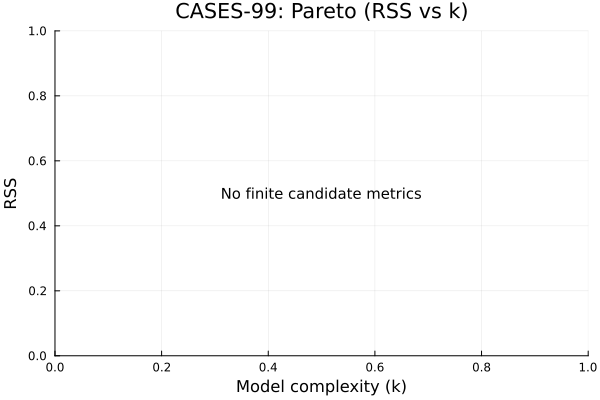
\includegraphics[width=\textwidth]{pde_benchmark/figures/cases_99_pareto_rss}
        \caption{CASES-99 Model Sparsity vs. RSS}
    \end{subfigure}
    \hfill
    \begin{subfigure}[b]{0.48\textwidth}
        \centering
        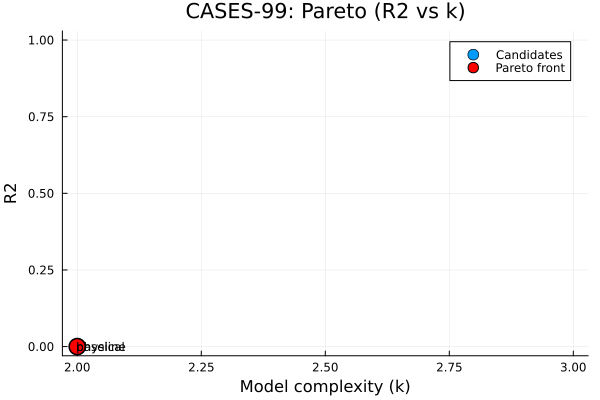
\includegraphics[width=\textwidth]{pde_benchmark/figures/cases_99_pareto_r2}
        \caption{CASES-99 Model Sparsity vs. $R^2$}
    \end{subfigure}
    \caption{Pareto trade-off frontiers between closure complexity ($k$) and goodness-of-fit metrics for CASES-99.}
    \label{fig:cases99_pareto}
\end{figure}

\subsection{SHEBA Pareto Closure Model}

The optimal discovered momentum closure for the Arctic SHEBA regime is given by:

\[
\frac{\partial u}{\partial t} = 32.1514\,\frac{\partial^{2} u}{\partial z^{2}}
\]


\begin{table}[H]
    \centering
    \caption{Discovered library terms and estimated sparse coefficients for SHEBA.}
    \label{tab:sheba_terms}
    \begin{tabular}{r l r}
\toprule
Term & Basis & Coefficient \\
\midrule
1 & $\frac{\partial^{2} u}{\partial z^{2}}$ & $3.94889$ \\
\midrule
\multicolumn{3}{l}{$R^{2} = 0.989577$} \\
\multicolumn{3}{l}{Residual norm = 0.484846} \\
\bottomrule
\end{tabular}
\end{table}

\begin{figure}[H]
    \centering
    \begin{subfigure}[b]{0.48\textwidth}
        \centering
        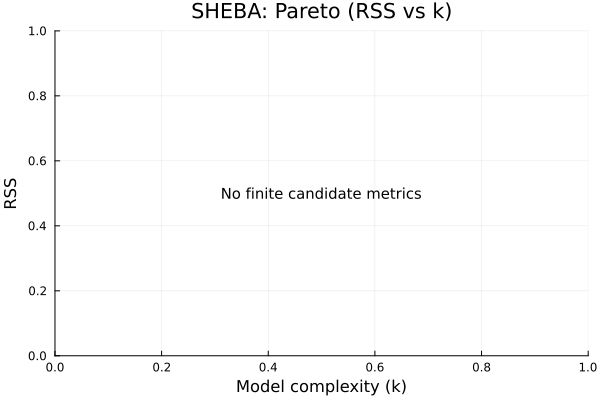
\includegraphics[width=\textwidth]{pde_benchmark/figures/sheba_pareto_rss}
        \caption{SHEBA Model Sparsity vs. RSS}
    \end{subfigure}
    \hfill
    \begin{subfigure}[b]{0.48\textwidth}
        \centering
        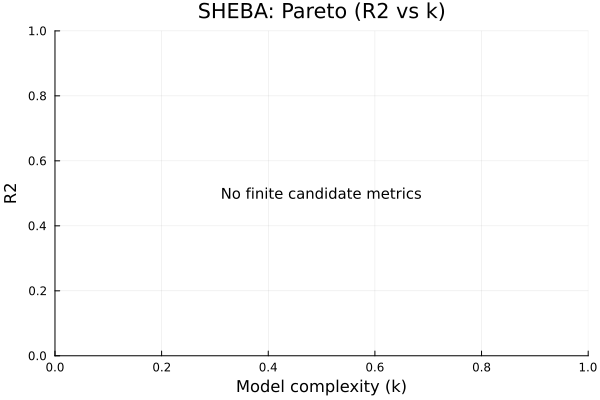
\includegraphics[width=\textwidth]{pde_benchmark/figures/sheba_pareto_r2}
        \caption{SHEBA Model Sparsity vs. $R^2$}
    \end{subfigure}
    \caption{Pareto trade-off frontiers between closure complexity ($k$) and goodness-of-fit metrics for SHEBA.}
    \label{fig:sheba_pareto}
\end{figure}

\subsection{Galerkin Modal Profile Comparisons}

Figure~\ref{fig:pde_profile_comp} compares terminal modal profile amplitudes produced by the discovered closures against initial observed profiles and neutral diffusion baselines.

\begin{figure}[H]
    \centering
    
\includegraphics[width=0.88\linewidth]{pde_benchmark/figures/pde_profile_comparison}
    \caption{End-state velocity profile comparisons across observed mean states, neutral baselines, and data-driven similarity closures.}
    \label{fig:pde_profile_comp}
\end{figure}

\end{document}